\chapter{Introduction}
\label{chap:introduction}


% \begin{figure}[H]
%   \center
%   \begin{tikzpicture}

%     \draw[fill=white!70!cyan] (1,0,0)--(7,0,0)--(8,1,0)--(0,1,0)--cycle;
%     \draw[fill=white!70!green] (2,-1,0)--(6,-1,0)--(7,0,0)--(1,0,0)--cycle;
%     \draw[fill=white!70!red] (3,-2,0)--(3.7,-4,0)--(4.3,-4,0)--(5,-2,0)--(6,-1,0)--(2,-1,0)--cycle;
%     %\draw[fill=white!70!cyan] (0,6,0)--(3,6,0)--(3,9,0)--(0,9,0)--cycle;

%     \draw[fill=red]  (4.5,-5,0) circle (0.3);
%     \draw[red, fill=red] (4.5,-5.3,0)--(4,-5.3,0)--(4,-4.7,0)--(4.5,-4.7,0)--cycle;
% 	\draw[fill=red] (4.5,-5.3,0)--(4,-5.3,0)--(4,-4.7,0)--(4.5,-4.7,0);
% 	\draw[fill=white] (3.5,-5,0) circle (0.3);
%     \draw[white, fill=white] (3.5,-5.3,0)--(4,-5.3,0)--(4,-4.7,0)--(3.5,-4.7,0)--cycle;
%     \draw[fill=white] (3.5,-5.3,0)--(4,-5.3,0)--(4,-4.7,0)--(3.5,-4.7,0);


%    \draw (4,1.5) node{\textasciitilde 1M composés} ;
%    \draw (4,0.5) node{\textasciitilde 10K composés} ;
%    \draw (4,-0.5) node{\textasciitilde 250 composés} ;
%    \draw (4,-1.5) node{\textasciitilde 5 composés} ;

%   \end{tikzpicture}
%     \caption{XXXXXXXXXX}
%     \label{fig:entonnoir_drug_design}
% \end{figure}



\begin{figure}[H]
  \center
  \begin{tikzpicture}

    \draw[fill=white!30!yellow] (0,1,0)--(3,3,0)--(3,9,0)--(0,11,0)--cycle;
    \draw[fill=white!30!orange] (3,3,0)--(6,4.5,0)--(6,7.5,0)--(3,9,0)--cycle;
    \draw[fill=white!30!red] (6,4.5,0)--(12,5.5,0)--(12,6.5,0)--(6,7.5,0)--cycle;


    \draw (-1.5,6) node[above]{\textasciitilde M} ;
    \draw (-1.5,6) node[below]{composés} ;
    \draw (1.5,6) node[above]{\textasciitilde 10K} ;
    \draw (1.5,6) node[below]{composés} ;
    \draw (4.5,6) node[above]{\textasciitilde 250} ;
    \draw (4.5,6) node[below]{composés} ;
    \draw (9,6) node[above]{\textasciitilde 5} ;
    \draw (9,6) node[below]{composés} ;
    
    \draw (1.5,11.5) node[above]{recherche et} ;
    \draw (1.5,11.5) node[below]{découverte} ;
    \draw (4.5,9.5) node[above]{développement} ;
    \draw (4.5,9.5) node[below]{pré clinique} ;
    \draw (9,8) node[above]{essais} ;
    \draw (9,8) node[below]{cliniques} ;

     \draw[fill=red]  (14.5,6,0) circle (0.3);
     \draw[red, fill=red] (14.5,6.3,0)--(14,6.3,0)--(14,5.7,0)--(14.5,5.7,0)--cycle;
  	 \draw[fill=red] (14.5,6.3,0)--(14,6.3,0)--(14,5.7,0)--(14.5,5.7,0);
     \draw[fill=white] (13.5,6,0) circle (0.3);
     \draw[white, fill=white] (13.5,6.3,0)--(14,6.3,0)--(14,5.7,0)--(13.5,5.7,0)--cycle;
     \draw[fill=white] (13.5,6.3,0)--(14,6.3,0)--(14,5.7,0)--(13.5,5.7,0);

     \draw[line width=2pt, latex-latex] (0,0) -- (3,0);
     \draw[line width=2pt, latex-latex] (3,0) -- (6,0);
     \draw[line width=2pt, latex-latex] (6,0) -- (12,0);

    \draw (1.5,0) node[below]{3 années} ;
    \draw (4.5,0) node[below]{1-2 années} ;
    \draw (9,0) node[below]{6-7 années} ;

  \end{tikzpicture}
    \caption{XXXXXXXXXX}
    \label{fig:entonnoir_drug_design}
\end{figure}



XXXXXXXXXXXXXXXXXXX dire que si on diminue le coût ça ouvre le marché vers d'autres médicaments XXXXXXXXXXXXXXXXXXXXXX 

Entre l'identification d'une cible thérapeutique et la mise sur la marché d'un nouveau médicament, une dizaine d'années de recherche et plus d'un milliard d’euros sont nécessaires [XXX REF]. Afin d'accélérer ce processus et ainsi d'en diminuer le coût, les simulations informatiques sont massivement utilisées. Pour s'approcher au maximum des conditions réelles, et donc de ce qu'il se passe dans le corps humain, ces simulations doivent avoir lieux dans l'eau, c'est à dire en solution. Malgré la puissance de calcul des ordinateurs actuels, ces simulations restent limitées à cause du nombre important de molécules d'eau nécessaires. Afin de s'adapter au mieux aux besoins des différentes études, il existe plusieurs représentations du solvant qui permettent de choisir entre vitesse et précision. Dans ce manuscrit, nous allons présenter la théorie de la fonctionnelle de la densité moléculaire (MDFT) qui allie vitesse et précision. Mon projet de thèse consiste à effectuer le premier pas vers toutes ces applications en adaptant la théorie ainsi que son implémentation aux systèmes biologiques.



\section{Contexte}
Avant d'envisager le développement d'une nouvelle solution thérapeutique il est nécessaire de comprendre les phénomènes à l'origine de la maladie que l'on souhaite guérir. La première étape consiste donc à comprendre la cascade biologique à l'origine de cette maladie. Une fois le phénomène identifié, les chercheurs vont sélectionner une protéine impliquée dans cette cascade. Cette molécule sera appelée "cible". A partir de cet instant, le développement d'un médicament va consister à trouver  parmi plusieurs millions de petits composés le meilleur candidat avant de l'optimiser. Ce candidat doit répondre à plusieurs critères: il doit (i) pouvoir accéder en quantité suffisante à la protéine cible, (ii) se lier à elle et l'inhiber afin de bloquer la cascade biologique à l'origine de la maladie visée et (iii) se lier le moins possible à d'autres protéines afin de minimiser les effets secondaires. Pour des raisons de sécurité, de temps et de coût, il est bien sur impossible de tester l'ensemble de ces millions de molécules en laboratoire ou en essai clinique. Les simulations informatiques sont donc massivement utilisées afin d'effectuer un premier tri et de passer de plusieurs millions de candidats à seulement quelques milliers. Les candidats ayant passés avec succès les différents tests (toxicité, affinité avec la cible, ...) seront ensuite synthétisés et testés en laboratoire. Une poignée de molécules prometteuses sera enfin testée en essai clinique. C'est seulement à l'issu de ce processus long et coûteux qu'une molécule pourra devenir un médicament. Tous ces phénomènes se déroulent dans le corps humain et donc en solution, le solvant aura donc un rôle clé dans l'ensemble de ces processus.



%Ces phénomènes se déroulent dans le corps humain et donc en solution, le solvant joue donc un rôle important dans le calcul de nombreux calculs et simulations que ce soit pour (i) permettre une meilleure compréhension de la cascade biologique à l'origine de la maladie visée ou (ii) pour guider la sélection des meilleurs candidats. 



\section{Solvatation}
La solvatation est le phénomène chimique qui consiste à plonger un composé, le soluté, qu'il soit solide, liquide ou gazeux dans une solution. Une fois en solution, la stabilité ainsi que le rôle du soluté seront fortement influencés par les molécules de solvant\cite{NickPace_protein_2004,levy_water_2004,Meyer_internal_1992,Ladbury_just_1996,GarcaSosa_hydration_2013,Lemieux_how_1996,Tame_role_1996,Li_effect_2005,Snyder_mechanism_2011,Wang_ligand_2011,Mobley_binding_2009,Barillari2007,Olano_hydration_2004,Bren_individual_2012,Ahmed_bound_2011,VAIANA_molecular_2006,Genheden_accurate_2011,Abel_contribution_2011,Biela_ligand_2012,Stegmann_thermodynamic_2009}. 

XXX Expérimentalement XXX



La façon de considérer le solvant au travers des simulations numériques reste un challenge actuel: En effet, par définition, les molécules de solvant sont prépondérantes dans la boite de simulation ce qui fait que la majorité du temps de calcul leur est consacré. Elles représentent donc le facteur limitant de la simulation. Pour dépasser les limites imposées pas une représentation explicite de ces molécules, des modèles implicites ont été proposés. Ces méthodes représentent le solvant sous la forme d'un milieu diélectrique continue. Le manque de détails moléculaire de ces méthodes comme les liaisons hydrogènes ou la gène stérique ne permet pas un calcul rigoureux des contributions entropiques. Malgré cela, une bonne paramétrisation leur à permis un développement rapide et efficace, avec parfois des prédictions d'énergies libres en bon accord avec les simulations numériques explicites pour des temps de calculs inférieurs de plusieurs ordres de grandeurs. 

La théorie des liquides constitue une 3$^{ème}$ approche, en particulier avec la théorie des équations intégrales, dans un premier temps avec une représentation atomistique. Quoi qu'il en soit, les équations intégrales sont difficiles, sensibles aux instabilités numériques et, d'après nos connaissances, limitées aux systèmes en 1 et 2 dimensions à l'exception des développements de Belloni et al. qui permettent l'étude de systèmes en quasi 3 dimensions, même si cela reste un secteur actuel de recherche. Une approximation de cette méthode à également été développée, le \textit{Reference interaction-site model} RISM, puis dérivée et adaptée aux solutés complexes en 3 dimensions 3DRISM. RISM et 3DRISM ont connue un grand succès car elles permettent de prédire les énergies libre de solvatation et les profils du solvant avec une précision acceptable, comme montré récemment sur des petites molécules neutres, des bio-molécules et même des ions [REF XXX]. Quoi qu'il en soit, ces méthodes considèrent les molécules de solvant comme un ensemble de sites corrélés entre eux, ce qui est schématiquement incorrect.

La théorie de la fonctionnelle de la densité moléculaire (MDFT) est encore une autre approche. Elle à des connections fortes avec la théorie des équations intégrales, mais est beaucoup moins sensible aux instabilités numériques car elle est basée sur la minimisation d'une fonctionnelle d'un problème variationnel. Le développement d'une fonctionnelle correcte reste cependant difficile et constitue un projet de recherche en cours. Le travail présenté dans ce manuscrit est basé sur cette théorie et son code associé. La MDFT nous fournit en quelques secondes seulement (quelques minutes pour les plus gros composés) deux paramètres essentiels à la compréhension des phénomènes ayant lieu en solution: l'énergie libre de solvatation et le profil de solvatation.



\begin{table}[H]
  \centering
  \begin{tabular}{ l | c c | c c }
    \hline & \\[-1em]\hline
    {} & \multicolumn{2}{|c|}{DM/MC} & MDFT & {}\\
    \hline
    Solvant    & explicite & implicite & hybride & {} \\
    \hline
    \multirow{2}{*}{Rapidité}   & \raisebox{-0.3\height}{
\includegraphics[width=0.03\textwidth]{chapters/introduction/images/moins.png}} & \raisebox{-0.3\height}{
\includegraphics[width=0.03\textwidth]{chapters/introduction/images/plus.png}} & \raisebox{-0.3\height}{
\includegraphics[width=0.02\textwidth]{chapters/introduction/images/plus.png}} & {} \\
    {}   & \raisebox{0.3\height}{({\raise.17ex\hbox{$\scriptstyle\mathtt{\sim}$}} jours)} & \raisebox{0.3\height}{({\raise.17ex\hbox{$\scriptstyle\mathtt{\sim}$}} secondes)} & \raisebox{0.3\height}{({\raise.17ex\hbox{$\scriptstyle\mathtt{\sim}$}} minutes)} & {} \\
    \hline
    Précision  & \raisebox{-0.2\height}{
\includegraphics[width=0.03\textwidth]{chapters/introduction/images/plus.png}} & \raisebox{-0.2\height}{
\includegraphics[width=0.03\textwidth]{chapters/introduction/images/moins.png}} & \raisebox{-0.3\height}{
\includegraphics[width=0.02\textwidth]{chapters/introduction/images/plus.png}} & {} \\
    
  \hline \multicolumn{5}{c}{} \\[-1em]\hline
  \end{tabular}
  \caption{Avantage et inconvénients principaux des différents type de solvant utilisés.}
  \label{tab:temps_calculs}  
\end{table}







\subsubsection{L'\'Energie libre de solvatation et structure du solvant}
L'énergie libre de solvatation correspond à l'énergie libre nécessaire au transfert de notre soluté depuis le vide jusqu'en solution. En d'autres termes, sur la figure \ref{fig:solvatation_def}, elle correspond à la différence d'énergie libre entre le système final (soluté en solution) et le système initial (soluté dans le vide + boite d'eau). L'énergie libre d'un système n'est pas directement calculable, elle se calcule comme la moyenne de boltzmann des énergies potentielles de l'ensemble des conformations possibles d'un système. Si on prend l'exemple d'une petite protéine de seulement 100 acides aminés et que l'on considère seulement 3 conformations par acide aminé. Le nombre de conformation possible est supérieur à 5e47. Pour chaque conformation obtenue, il faut prendre en compte toutes les conformations possibles de la chaîne principale. Et pour chaque conformation de la chaîne principale, il faut également prendre en compte toutes les conformations possibles pour les milliers de molécules d'eau qui l'entour. Il est donc impossible de prendre en compte numériquement l'ensemble de ces conformations. Afin de rendre ces calculs possibles, différentes approximations, plus ou moins précises, de ce calcul ont été proposées.


\begin{figure}[h]
  \center
  \begin{tikzpicture}
  \tikzstyle{lien}=[->,>=stealth,rounded corners=5pt,thick]
  \node[inner sep=0pt] (prot) at (0,0)
      {\setlength{\fboxrule}{1pt}%
      {\fbox{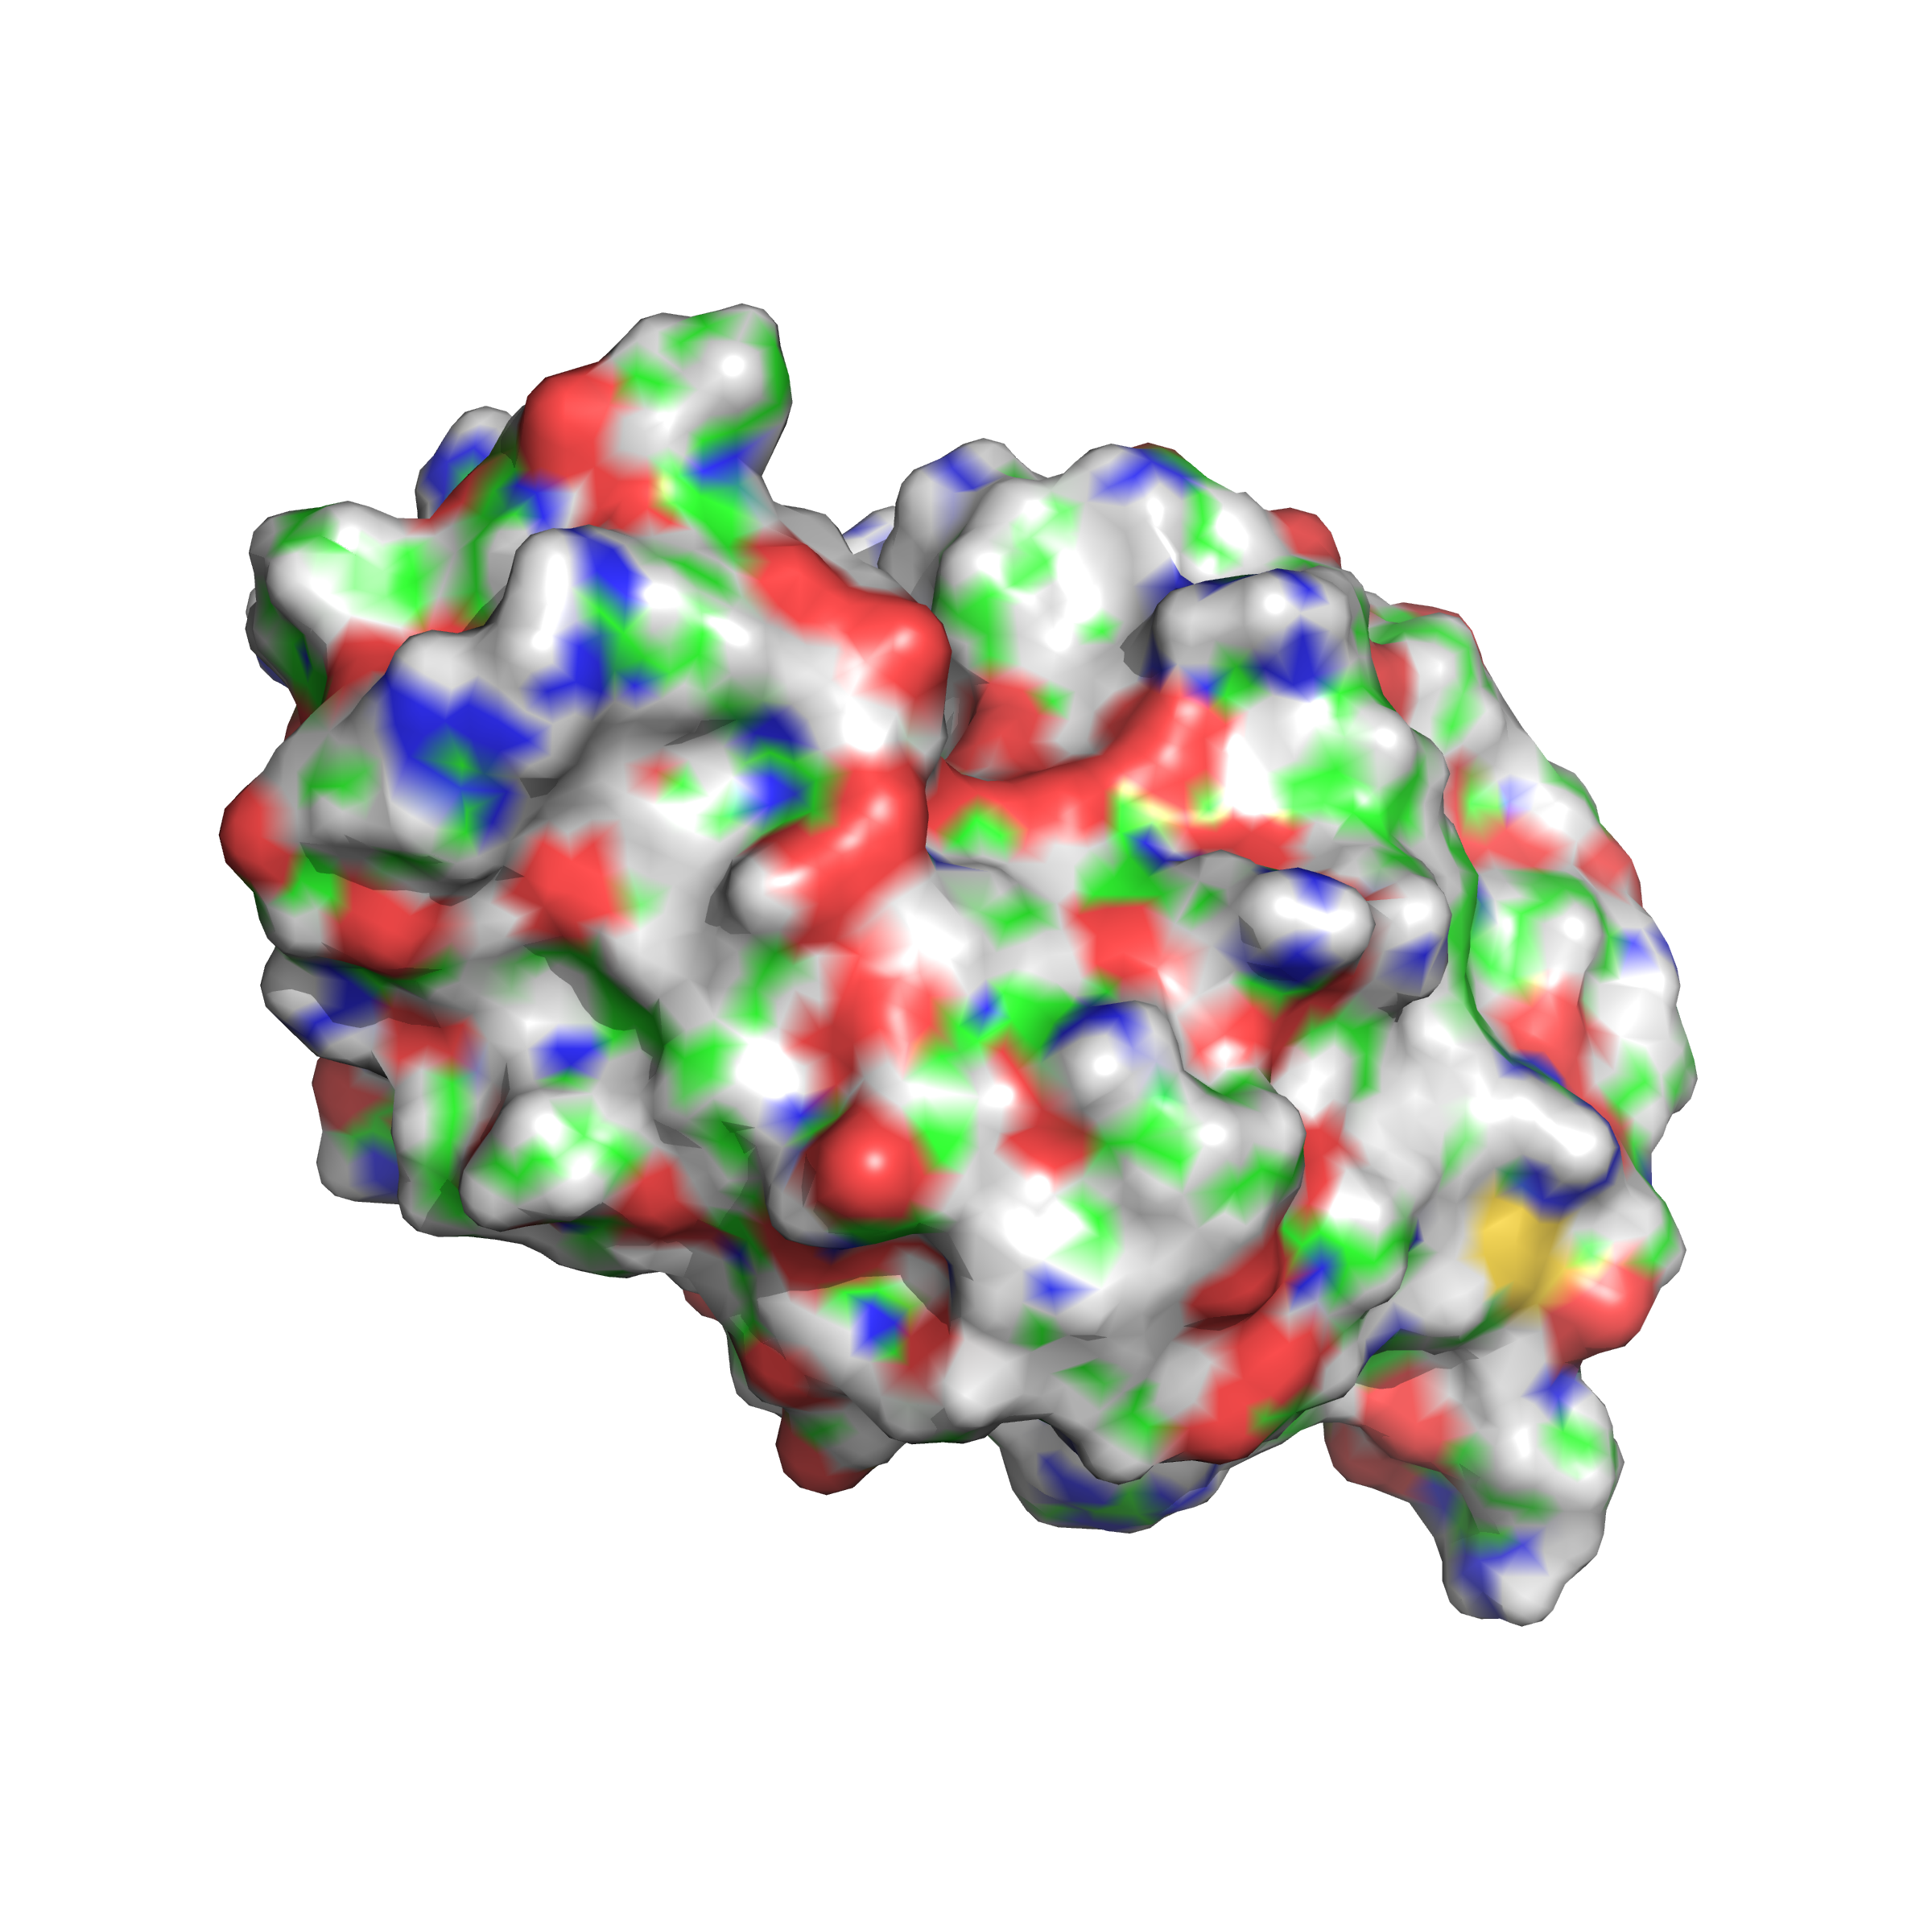
\includegraphics[width=.25\textwidth]{chapters/introduction/images/prot.png}}}%
      };
  \node[inner sep=0pt] (water) at (6,0)
      {\setlength{\fboxrule}{1pt}%
      {\fbox{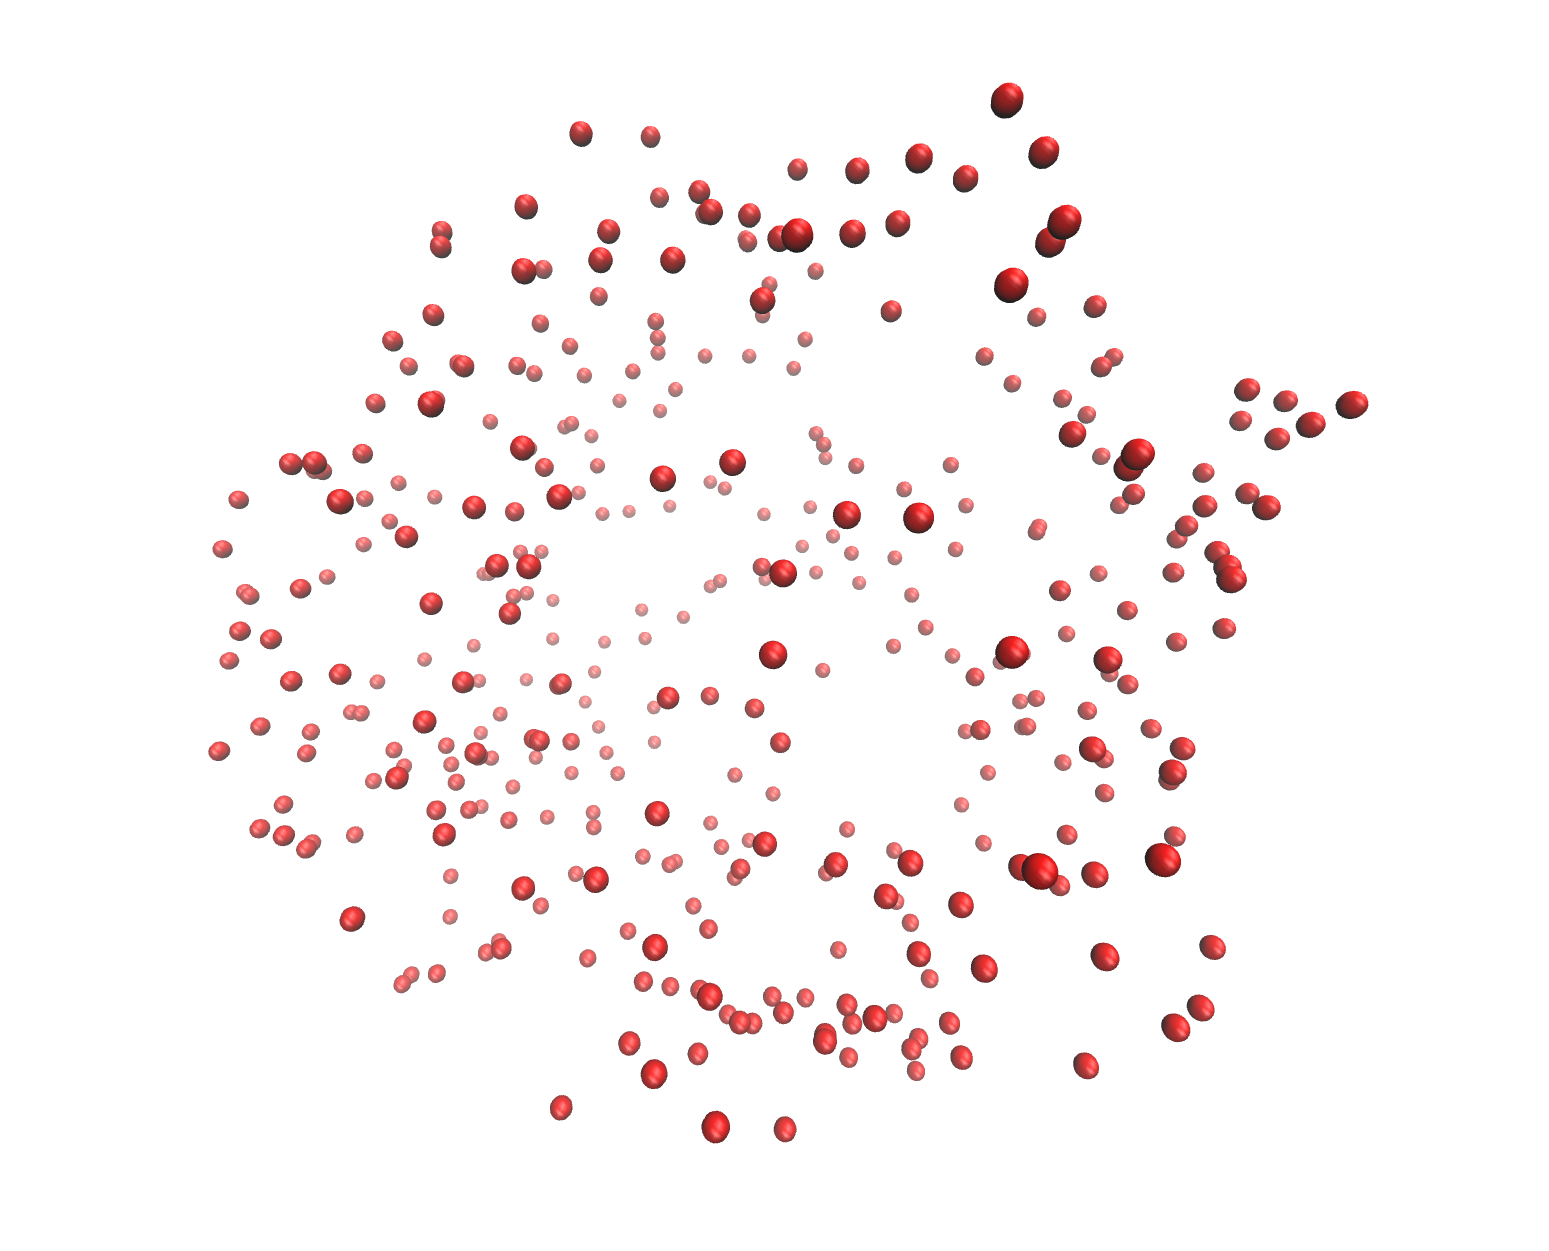
\includegraphics[width=.25\textwidth]{chapters/introduction/images/water.png}}}%
      };
  \node[inner sep=0pt] (prot_water) at (12,0)
      {\setlength{\fboxrule}{1pt}%
      {\fbox{\includegraphics[width=.25\textwidth]{chapters/introduction/images/prot_water.png}}}%
      };

  \draw (2.5,0) node[right] {+};

  \draw[-latex] (water) -- (prot_water);
  
  \end{tikzpicture}
      \caption{Solvatation d'une protéine.}
      \label{fig:solvatation_def}
\end{figure}



\subsubsection{Les méthodes explicites}
Les méthodes les plus rigoureuse sont couplés à des simulations de dynamique moléculaire (MD) ou monte carlo (MC) pour lesquelles le solvant est représenté de façon explicite. Parmi les méthodes existantes\cite{Skyner_review_2015, Hansen_Practical_2014, Christ_basic_2009}, on peut citer l'intégration thermodynamique (TI) ou encore la méthode de perturbation d'énergie libre (FEP). Afin de simuler une transition lente de l'état initial à l'état final, une vingtaine de simulations de dynamique moléculaire (MD) ou monte carlo (MC) sont lancées. Chacune d'entre elle représente un état intermédiaire de la transformation étudiée. Une fois l'ensemble des simulations terminées, l'énergie libre de la transformation étudiée correspond à la somme des moyennes de la différence d'énergie potentielle entre deux états voisins. Elle s'écrit sous la forme

\begin{eqnarray}
\Delta F(A \rightarrow B) =  \int_0^1 \left\langle U_B(\lambda) - U_A(\lambda) \right\rangle_{\lambda} d\lambda
\end{eqnarray}

Ces calculs, très précis, fournissent une énergie libre de solvatation ainsi qu'une image précise de l'organisation su solvant autour de notre soluté au prix de plusieurs jours de calculs.



\subsubsection{Les méthodes implicites}
Pour des résultats nécessitant une moins bonne précision, des méthodes rapides, basées sur une représentation implicite du solvant ont été proposées\cite{Skyner_review_2015}. Le solvant implicite est généralement couplé aux méthodes PBSA ou GBSA. Ces méthodes très simplifiées fournissent un résultat quasi instantanément. Pour cela, la partie électrostatique est prise en charge en résolvant dans un cas, l'équation de Poisson (P) et dans l'autre cas l'équation de Born généralisée (GB). L'hydrophobicité (la création de la cavité) est quant à elle prise en compte via la surface accessible au solvant (SA). L'énergie libre de solvatation correspond ensuite à une simple combinaison linéaire de ces deux termes. Le succès de ces méthodes est dû à une bonne paramétrisation de ces termes. Ces deux méthodes, couplées à des énergies de mécanique moléculaire, donnent lieux à des méthodes  populaires du calcul de l'énergie libre de liaison en solution. Ces méthodes, MM/PBSA\cite{Genheden__MMPBSA_2015} et MM/GBSA seront développées dans le chapitre XXX.

Contrairement aux méthodes explicites, ces méthodes ne fournissent aucune informations sur l'organisation du solvant.


\subsubsection{Les méthodes dérivées de la théorie des liquides}
Parmi les méthodes issues de la théorie des liquides, nous nous intéresserons ici à la théorie de la fonctionnelle de la densité moléculaire (MDFT). Cette théorie calcul l'énergie libre de solvatation ainsi que la structure du solvant en quelques secondes seulement et avec une précision comparable aux méthodes explicites. Cette théorie est décrite en détaille dans le chapitre suivant.




\subsection{Quelques exemples}
Ce paragraphe n'a pas vocation à être exhaustif mais simplement à montrer au travers de quelques exemples l'importance de ces paramètres. On considère dans un premier temps la structure du solvant. L'importance de l'eau dans la stabilité et le rôle des protéines n'est plus à démontrer[REF XXX], cette information est donc capitale à la compréhension des mécanismes à l'origine d'une maladie. De la même manière, l'eau en créant un réseau de liaison hydrogènes, aura une influence non négligeable sur l'affinité et donc la stabilité des interactions entre deux composés. Cette information permet donc par exemple d'optimiser un candidat médicament. C'est ce qu'on fait XXX et Al. [REF watermap XXX] dans leur étude. Ils ont calculé l’entropie de chaque molécule d'eau se situant à proximité des interactions. Des fragment ont ensuite été ajoutés à ce ligand (médicament), de façon à venir prendre la place des ces molécules d'eau très énergétiques. En diminuant l'énergie globale du système ils ont ainsi favorisé cette liaison et donc augmenté l'efficacité de ce composé.

L'énergie libre de solvatation peut quant à elle être dérivée en de nombreuses autres grandeurs. Dans les cas des médicaments administrables par voie orale, Lipinski et Al. [REF XXX] ont défini la \textit{régle des 5} qui comporte un ensemble de 4 critères qu'elles doivent respecter. Si une petite molécule ne respecte pas l'ensemble de ces 4 règles, ses chances qu'elles deviennent un jour un médicament oral sont très faibles. Pour respecter ces critères, cette molécule doit posséder au maximum 5 donneurs de liaison hydrogènes, au maximum 10 accepteurs de liaisons hydrogènes, une masse moléculaire inférieure à 550 daltons et un logP inférieur à 5. Si les 3 premiers paramètres peuvent être calculés directement, ce n'est pas le cas du dernier. Le logP correspond au logarithme du rapport entre la solubilité du composé dans l'eau et dans l'octanol. Il peut donc être dérivé des énergies libre de solvatation de ce composé dans ces deux solvants. L'énergie libre de solvatation, couplée à des calculs de mécanique moléculaire permet également de simplifier le calcul de l'énergie libre de liaison. La méthode MM/PBSA\cite{Genheden__MMPBSA_2015} est décrite et dérivée en MM/MDFT dans le chapitre XXX. Enfin on peut citer également le calcul du logBBB (coefficient de partition entre le cerveau et le sang). Dans le cas des maladies neurologiques, le médicament doit pouvoir atteindre le cerveau et donc traverser la barrière hémato-encéphalique. Pour cela, le logBBB doit être compris entre -1 et 0.3 [REF XXX]. Ce paramètres peut également être dérivé de la valeur de l'énergie libre de solvatation comme l'on montré Lombardo et al\cite{Lombardo_computation_1996}.

Dans ce paragraphe nous ne présentons qu'une petite partie des possibilités qu'offre une représentation rapide et efficace de la solvatation comme le propose MDFT. Mon projet de thèse consiste à effectuer le premier pas vers toutes ces applications en adaptant la théorie ainsi que son implémentation aux systèmes biologiques.




\vspace{8\baselineskip}

\boitemagique{A retenir}{
Dans ce chapitre nous introduisons le contexte de cette thèse et présentons l'état de l'art des méthodes de solvatation. Nous montrons également en quoi l'énergie libre de solvatation et la structure du solvant sont omniprésentes tout au long du développement et de l'optimisation d'un médicament. 
}



